\documentclass[12pt]{article}
\usepackage[utf8]{inputenc}
\usepackage[left=2.5cm,right=2.5cm,top=2.5cm,bottom=2.5cm]{geometry}
\usepackage{cite}

\usepackage{amsmath,amssymb,amsfonts,amsthm}
\newtheorem{theorem}{Theorem}
\newtheorem{cor}[theorem]{Corollary}
\newtheorem{lemma}[theorem]{Lemma}
\newtheorem{conjecture}[theorem]{Conjecture}
\newtheorem{prop}[theorem]{Proposition}
\newtheorem{claim}{Claim}
\theoremstyle{definition}
\newtheorem{definition}{Definition}
\newtheorem{remark}{Remark}
\newtheorem{assumption}{Assumption}
\newtheorem{corollary}{Corollary}
\newtheorem{example}{Example}
\DeclareMathOperator*{\argmax}{arg\,max}
\DeclareMathOperator*{\argmin}{arg\,min}

\usepackage{gensymb}
\usepackage{graphicx}
\usepackage{multirow}
\usepackage{multicol}
\usepackage{caption}
\usepackage{comment, bm, enumerate}
\usepackage[ruled,vlined]{algorithm2e}
\usepackage{wrapfig}
% Example for wrapping text around a figure 
% \begin{wrapfigure}{R}{0.3\textwidth}
% \centering
% \includegraphics[width=0.25\textwidth]{path_to_your_figure}
% \caption{\label{label_of_your_figure}This is a figure caption.}
% \end{wrapfigure}

\usepackage{subfig}
% Example for including multiple images into one figure
% \begin{figure}
%      \centering
%      \begin{subfigure}[b]{0.3\textwidth}
%          \centering
%          \includegraphics[width=\textwidth]{path_to_your_graph1}
%          \caption{caption_of_your_graph1}
%          \label{label_of_your_graph1}
%      \end{subfigure}
%      \hfill
%      \begin{subfigure}[b]{0.3\textwidth}
%          \centering
%          \includegraphics[width=\textwidth]{path_to_your_graph2}
%          \caption{caption_of_your_graph2}
%          \label{label_of_your_graph2}
%      \end{subfigure}
%      \hfill
%      \begin{subfigure}[b]{0.3\textwidth}
%          \centering
%          \includegraphics[width=\textwidth]{path_to_your_graph3}
%          \caption{caption_of_your_graph3}
%          \label{label_of_your_graph3}
%      \end{subfigure}
%         \caption{Three graphs example}
%         \label{fig:three graphs}
% \end{figure}

\usepackage[dvipsnames]{xcolor}
\usepackage[T1]{fontenc}
\usepackage{hyperref}
\hypersetup{
    colorlinks=true,
    linkcolor=blue,
    filecolor=magenta,      
    urlcolor=cyan,
    pdftitle={Overleaf Example},
    pdfpagemode=FullScreen,
}

\usepackage{booktabs, caption, makecell}
\usepackage{threeparttable}

\usepackage{listings}
\lstset{basicstyle=\footnotesize\ttfamily,breaklines=true}
\lstset{framextopmargin=50pt,frame=bottomline}
% Default BibTeX in apalike style, activate the following line:
\bibliographystyle{apalike}

% If you use natbib package, activate the following three lines:
%\usepackage[round]{natbib}
%\renewcommand{\bibname}{References}
%\renewcommand{\bibsection}{\subsubsection*{\bibname}}

\title{Clustering Single Cell RNA Sequencing Data Based on Gaussian Mixture Model}
\author{CompSci 671\\
Jingxuan Zhang}
\date{Dec 10, 2021}

\begin{document}
\maketitle

\section{Background}
\subsection{Introduction}

The cell, as the fundamental unit and functional base to build the human body, is often treated as the target object in numerous biological studies. Due to the process of cell differentiation, cells are grown into different cell types and implement different functions. Therefore, identifying cell types somehow becomes a prior goal for downstream analysis in the following studies and bioinformaticians has made many efforts to find ways to do so. At the beginning, the microscope helped distinguish cells by the size, shape and structure. Later, investigators tended to use biological markers to determine the appearance or distribution of the surface protein on the cell membrane and identify cell types based on this pipeline [1]. However, these methods seem to have a very low power to classify cells and the poor performance may be due to the tiny fraction of the proteome that can be reflected by the structures or the membrane protein of the cells [1].

To obtain and utilize the full information from gene expressions, new methods should seek other products in the central dogma of molecular biology, which is RNA. Hopefully, with the development in RNA extraction and amplification methods, RNA-seq data soon became available in lab research. Along with the application of digital microfluidics to isolate cells from sample tissues, the first single-cell RNA sequencing (scRNA-seq) experiment was completed in 2009 and since then many more sequencing data were obtained, most of which were collected through 10X Genomics [2].

Contemporarily, researchers are working to design efficient and well-performed algorithms to classify cells into different cell types. In this sense, unsupervised clustering methods provide some good choices to fulfill this function. Traditional unsupervised clustering methods such as hierarchical clustering and k-means method often bring a relatively unsatisfying performance on raw count data because of the high dimensionality and high sparsity in RNA-seq data. To handle this problem, researchers need to apply PCA before applying these methods [1]. However, this will increase the impact of noise from low-expressed genes that are expected to be rare in most of the cell types. Moreover, if the number of genes included in the dataset is large, these methods will cause a high computational burden and no longer be efficient [3].


\subsection{Related Work}

Hierarchical clustering is a traditional method that sequentially combines individual cells into larger clusters (agglomerative) or divides clusters into smaller groups (divisive) [1]. This method can be applied to raw count data as well as the transformed data matrix after PCA. One of the most common linkages for RNA-seq data is Wald.D2 and it will be implemented in this project. An important shortcoming is that both time and memory requirements scale quadratically with the number of cells increasing. Another disadvantage is that there is no agreement on how to find methods to determine the division level where we cut the tree. Therefore, we will cut the tree manually, which may not optimize the final performance on this method.

Another common clustering method is k-means which utilizes Lloyd’s algorithm iteratively identifies k cluster centres (centroids) where k should be pre-specified, and each cell is assigned to the closest centroid [1]. Since it has the advantage of scaling linearly with the number of points, it can also be applied to either raw count data or the transformed data matrix after PCA. The method to specify the number of clusters is usuallly based on gap statistics. However, Lloyd’s algorithm is greedy, which means that it cannot guarantee to find the global minimum [1]. This drawback is overcome by repeated application of k-means using different initial conditions or upstream processing and finding the consensus, as performed by SC3 [3]. Another disadvantage of k-means is its bias towards identifying equal-sized clusters, which may result in rare cell types being hidden among a larger group. To overcome these issues, RaceID augments k-means with outlier detection to identify rare cell types [4].

Many researchers also prefer to use KNN algorithm because it can be easily implemented and more intuitive in the way to classify data points. For example, one of the most popular clustering methods for scRNA-seq data is the shared nearest neighbor (SNN) method which is just a one-step extension based on k-nearest neighbor (KNN) algorithm. This method is implemented in “Seurat” package in R and can be applied to multiple types of data, including single-cell multimodal data [5]. Instead of treating each cell equally as KNN does, the procedure chooses to set different weights to each pair of cells after computing their distance [3]. This will lead to a SNN graph. More specifically, for each cell, SNN graph will connect (assign an edge) between relatively similar cells according to the similarity matrix and then add weight to each edge based on some certain function. This approach consists of two steps: 1. Constructing the SNN graph. 2. Clustering based on the SNN graph. More details can be referred to the open-source R package Seurat (https://www.github.com/satijalab/seurat).

 


\section{Methods}

\subsection{Model}

The model designed for this project is based on Gaussian Mixture Model (GMM). Gaussian mixture models are a probabilistic model that helps to represent normally distributed subpopulations within a whole population. Since it applies EM algorithm to update the centroids in order to optimize the likelihood function and finally returns the probability of each data points that are given from certain cluster, the Gaussian mixture model (GMM) is also commonly implemented in classification problems. However, it is developed to estimate the density function of the data with the normality operating assumption. Therefore, in the case of high and collinear process variables, learning from data with GMM can be difficult or impossible [6].

ScRNA-seq data contains all the count of genes as rows for each cell as columns. Therefore, the normality assumption does not match. In addition, the count matrix will have other properties that are quite unique in sequencing data. For example, high dimensionality and high sparsity are often described as the key features for this type of dataset and should be carefully handled when designing the clustering algorithm. Therefore, a zero-inflated dimensional reduction process should be applied in order to improve the computational efficiency while removing out the noise. Moreover, it can help transform the data to make it satisfy the normality assumption for GMM.

To implement this dimensional reduction process, I choose to apply (Z)ero (I)nflated (F)actor (A)nalysis (ZIFA). This method handles the high-dimensional data and tries to transform the data to a low-dimensional latent space. Meanwhile, it considers dropout event that leads the single-cell gene expression data to containing false zero expression. Each subject in the study $Y_i$ is assumed to be independent and $Z_i$ is the random variable that contains the corresponding information in latent space. Details in derivations is shown below, $i=1,...,N$ is for the index over samples (cells), $j=1,...,D$ is for the index over genes and $k=1,..., K$ is for the index over latent dimensions [7].
\begin{align}
    \bm{z}_i & \sim N(\bm{0}, \bm{I})\\
    \bm{x}_i | \bm{z}_i & \sim N(\bm{A}\bm{z}_i+\bm{\mu}, \bm{W})\\
    h_{ij} | x_{ij} & \sim Bernoulli(p_{ij})\\
    p_{ij} & =\exp(-\lambda x^2_{ij})\\
    y_{ij} & = \begin{cases}
      x_{ij} & \text{if $h_{ij} = 0$}\\
      0 & \text{otherwise}
    \end{cases}     
\end{align}

The function is realized by EM algorithm to find the optimal parameters ($\bm{A}$, $\bm{\mu}$, $\bm{W}$ and $\lambda$) and can be directly called from the package from (https://github.com/epierson9/ZIFA) [7].

\subsection{Hyper-parameter Selection}
The hyper-parameter for this model is the dimension of the latent space into which the original read count data are projected. It should not be too small because it cannot extract all the important information from the original data. Also, a large dimension for latent space will also include more noise. Usually, most of the previous studies tend to set $K$ between $50$ and $100$ and we would select $50$ to alleviate the computational burden.

\section{Experiments}
\subsection{Experimental Setup}

The single cell RNA-seq data analyzed in this paper were collected from female mice between $6-10$ weeks for experimental procedures. The researchers applied tumor-inducing doses titration of 4T1 cells and injected 100 4T1 cells into the mice in order to nourish certain tumors in 3
weeks. They also ensured not to visibly detect 4T1 carcinoma in lung of these mice until 5 weeks to ensure no metastases occurred. Afterwards, single cell techniques were implemented for dissociate and homogenize the tumor tissues. T-cells which is the focus in this project were filtered out and sequenced by 10X Genomics [8]. During the pre-processing stage, genes whose expression level was zero across more than $2\%$ of the cells and cells that had less than $2\%$ of the genes expressed were removed. As a result, the read count matrix totally consists of $2,989$ cells as rows and $7,893$ genes as columns. Since there are two cells that have the same cell ID with multiple cell type labels, they will not be included in this study for clustering analysis. The remaining T-cells are eventually classified into five cell subtypes. The benchmark labels are provided for verification, so it is interesting to design and compare methods to cluster these T-cells based on the read count matrix considering its characteristics, like high sparsity and high dimensionality. Fiugre 1 shows the proportions of each cell subtype labels.

\subsection{Evaluation Metrics}
To obtain and compare the performance across different clustering algorithms on this scRNA-seq dataset after dimensional reduction procedure by PCA or ZIFA, I assign each cluster to the class with the majority label. In other words, the predicted cell type label for each cluster is determined by the majority of the cells in this cluster and we could then compute the label predicting accuracy through all the 2,985 cells involved in this project (shown in Figure 1). Furthermore, the processing time for each algorithms is also recorded in Figure 2 to help compare the running efficiency across different methods.

\subsection{Experimental Results}

\begin{figure}[h]
    \centering
    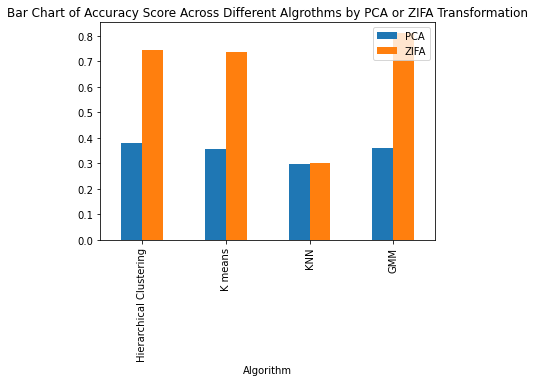
\includegraphics[scale=0.75]{Figure 1.png}
    \caption{Grouped Bar Chart of Accuracy Score}
    \label{fig:mesh1} the \\
    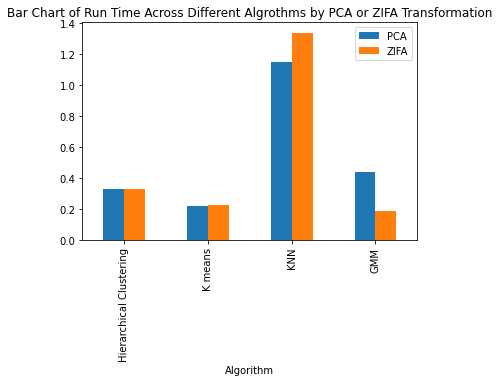
\includegraphics[scale=0.75]{Figure 2.png}
    \caption{Grouped Bar Chart of Run Time in Seconds}
    \label{fig:mesh1}
\end{figure}

From Figure 1, it is clear to find that Gaussian mixture method along with ZIFA dimensional reduction algorithm has the best performance in accuracy score that achieves more than $80\%$ on this scRNA-seq dataset. Moreover, except for KNN clutering method, ZIFA attains a significant improvement in the performance comparing to PCA, the traditional dimensional reduction approach. This is not unexpected because I have point out the high sparsity feature of this dataset, which makes it more reasonable to build a zero-inflated model when projecting the count data to a lower dimensional space. Figure 2 presents the run time for each method, where all the coding is processed under the same condition (a single CPU and 32GB RAM). As a result, GMM along with ZIFA also wins the highest efficiency in this process. However, the recorded time is merely for the process of each clustering method on certain transformed data. While comparing to PCA that only needs a few seconds to extract the first 50 components, the running time for ZIFA is more than 40 mins for this dataset and could be roughly linear with respect to the number of samples and the number of genes. This is because ZIFA needs to apply EM algorithms during this procedure, which brings huge computational burdens and may need further improvement in future.

\section{Errors and Mistakes}

I try to set the number of clusters equal to 5 (or close to 5 for KNN), but this may not be realistic. In most real cases, we cannot know the exact or optimal number of clusters because the true labels are often unknown. Therefore, many clustering algorithms designing for analyzing scRNA-seq data tend to be over-clustering. Then it may separate a same cell type into multiple clusters. Meanwhile, they need to build regression models to help discover the differentially expressed genes within each cluster and utilize biological knowledge to relabel the clusters. This implementation will definitely improve the accuracy when classifying cells into differnet cell types. Imagine the most extreme case that each cell is clustered to a different cluster respectively. As a consequence, it achieves highest accuracy but lets the algorithm the most useless. The determination of the number of clusters across all unsupervised methods is a general problem, but it has not reached an agreement among researchers and may become a future direction to work on beyond this project.

\section*{Citations}
1. Kiselev, V. Y., Andrews, T. S., & Hemberg, M. (2019, January 7). Challenges in unsupervised clustering of single-cell RNA-seq data. Nature News. Retrieved November 3, 2021, from https://www.nature.com/articles/s41576-018-0088-9. 

2. Hao, Y., Hao, S., Andersen-Nissen, E., Mauck, W. M., Zheng, S., Butler, A., Lee, M. J., Wilk, A. J., Darby, C., Zager, M., Hoffman, P., Stoeckius, M., Papalexi, E., Mimitou, E. P., Jain, J., Srivastava, A., Stuart, T., Fleming, L. M., Yeung, B., … Satija, R. (2021). Integrated Analysis of multimodal single-cell data. Cell, 184(13). https://doi.org/10.1016/j.cell.2021.04.048 

3. Kiselev, V. Y., Kirschner, K., Schaub, M. T., Andrews, T., Yiu, A., Chandra, T., Natarajan, K. N., Reik, W., Barahona, M., Green, A. R., amp; Hemberg, M. (2017). SC3: Consensus clustering of single-cell RNA-seq data. Nature Methods, 14(5), 483–486. https://doi.org/10.1038/nmeth.4236

4. Gru ̈n, D., Lyubimova, A., Kester, L., Wiebrands, K., Basak, O., Sasaki, N., Clevers, H., amp; van Oudenaarden, A. (2015). Single-cell messenger RNA sequencing reveals rare intestinal cell types. Nature, 525(7568), 251–255. https://doi.org/10.1038/nature14966

5. Xu, C., & Su, Z. (2015). Identification of cell types from single-cell transcriptomes using a novel Clustering Method. Bioinformatics, 31(12), 1974–1980. https://doi.org/10.1093/bioinformatics/btv088 

6. Nada A. Alqahtani, Zakiah I. Kalantan, "Gaussian Mixture Models Based on Principal Components and Applications", Mathematical Problems in Engineering, vol. 2020, Article ID 1202307, 13 pages, 2020. https://doi.org/10.1155/2020/1202307

7. Pierson, E., Yau, C. ZIFA: Dimensionality reduction for zero-inflated single-cell gene expression analysis. Genome Biol 16, 241 (2015). https://doi.org/10.1186/s13059-015-0805-z

8. Christian, L. S., Wang, L., Lim, B., Deng, D., Wu, H., Wang, X.-F., &amp; Li, Q.-J. (2021). Resident memory T&nbsp;cells in tumor-distant tissues fortify against Metastasis Formation. Cell Reports, 35(6), 109118. https://doi.org/10.1016/j.celrep.2021.109118 

\section*{Code}
\begin{lstlisting}
# Import packages
import pyreadr
import pandas as pd
import numpy as np
import matplotlib.pyplot as plt
import timeit


# Pacakges for dimensional reduction procedure
from sklearn.decomposition import PCA
from ZIFA import ZIFA
from ZIFA import block_ZIFA

# Pacakges for different clustering method
# Hierarchical Clustering
from sklearn.cluster import AgglomerativeClustering
# K Means
from sklearn.cluster import KMeans
# KNN
from sklearn.neighbors import NearestNeighbors
# Gaussian Mixture Model
from sklearn.mixture import GaussianMixture

from sklearn.metrics import accuracy_score


# Set random seed
import random
random.seed(25)

## Import data from rds file
count = pyreadr.read_r('../Data/Tcell_5type_filtered.rds')
count = count[None]
label = pyreadr.read_r('../Data/Tcell_5type_filtered_labels.rds')
label = label[None]

# Extract the read count array
count_array = count.to_numpy()

# Change labels to integer
new_cluster = dict(zip(list(set(label['Group'])), list(range(5))))
new_label = []
for k in range(len(list(label['Group']))):
    old_label = list(label['Group'])[k]
    new_label.append(new_cluster[old_label])
    
## Implement PCA
pca = PCA(n_components=50)
count_array_pca = pca.fit_transform(np.transpose(count_array))

# Check the dim of the array after PCA transformation
count_array_pca.shape

## ZIFA
# compute the log count array by log2(1 + count_data)
log_count_array = np.log(1 + count_array)

count_array_ZIFA, model_params = block_ZIFA.fitModel(np.transpose(log_count_array), 50, p0_thresh=0.9)

# Store the array to avoid multiple running and save time
# Since it takes more than 40 mins to run this procedure, I save the result to a csv file for convenience.
pd.DataFrame(count_array_ZIFA).to_csv("count_array_ZIFA.csv")

# Check the dim of the array after ZIFA transformation
count_array_ZIFA.shape


## Hierarchical Clustering
start = timeit.default_timer()

# Hierarchical Clustering on PCA array
hc_pca = AgglomerativeClustering(n_clusters=5).fit(count_array_pca)
# Obtain Predicted labels
hc_pca_pred = hc_pca.labels_

stop = timeit.default_timer()
# Record Run time
hc_pca_time = stop - start

start = timeit.default_timer()

# Hierarchical Clustering on ZIFA array
hc_ZIFA = AgglomerativeClustering(n_clusters=5).fit(count_array_ZIFA)
# Obtain Predicted labels
hc_ZIFA_pred = hc_ZIFA.labels_

stop = timeit.default_timer()
# Record Run time
hc_ZIFA_time = stop - start


## K means
start = timeit.default_timer()

# K Means on PCA array
kmeans_pca = KMeans(n_clusters=5, random_state=0).fit(count_array_pca)
# Obtain Predicted labels
kmeans_pca_pred = kmeans_pca.labels_

stop = timeit.default_timer()
# Record Run time
kmeans_pca_time = stop - start

start = timeit.default_timer()

# K Means on ZIFA array
kmeans_ZIFA = KMeans(n_clusters=5, random_state=0).fit(count_array_ZIFA)
# Obtain Predicted labels
kmeans_ZIFA_pred = kmeans_ZIFA.labels_

stop = timeit.default_timer()
# Record Run time
kmeans_ZIFA_time = stop - start


## KNN
def gather_neighbors(tree):
    """
    This function is used to gather neigbors which is the output from TreeBall algorithm and 
    make them in the same cluster.
    """
    tree_list = list(tree)
    cluster = []
    i = len(tree_list)
    while(len(tree_list) > 0):
        cluster.append(np.array(tree_list[-1]))
        n_old = 0
        n_new = len(tree_list)
        while (n_old != n_new):
            # When no update in tree_list, which means that the union of neighborhoods based on the initial 
            # neighborhood is complete. Then break the inner while loop and initialize with a new neighborhood.
            for j in range(n_new - 1, -1, -1):
                # Use for loop to determine if two neighborhoods share same data points, union them.
                if len(set(tree_list[j]).intersection(set(cluster[-1]))) > 0:
                    cluster[-1] = np.array(list(set(tree_list[j]).union(set(cluster[-1]))))
                    tree_list.pop(j)
            n_old = n_new
            n_new = len(tree_list)
        
    return cluster
    
start = timeit.default_timer()

# KNN on PCA array
neigh = NearestNeighbors(n_neighbors=3)
neigh.fit(count_array_pca)
a = neigh.kneighbors(count_array_pca, return_distance=False)
cluster_pca = gather_neighbors(a)
len(cluster_pca)
# Obtain Predicted labels
knn_pca = np.zeros(count_array_pca.shape[0])
for i in range(len(cluster_pca)):
    for j in cluster_pca[i]:
        knn_pca[j] = i
knn_pca

stop = timeit.default_timer()
# Record Run time
knn_pca_time = stop - start

start = timeit.default_timer()

# KNN on PCA array
neigh = NearestNeighbors(n_neighbors=3)
neigh.fit(count_array_ZIFA)
b = neigh.kneighbors(count_array_ZIFA, return_distance=False)
cluster_ZIFA = gather_neighbors(b)
len(cluster_ZIFA)
# Obtain Predicted labels
knn_ZIFA = np.zeros(count_array_ZIFA.shape[0])
for i in range(len(cluster_ZIFA)):
    for j in cluster_ZIFA[i]:
        knn_ZIFA[j] = i

stop = timeit.default_timer()
# Record Run time
knn_ZIFA_time = stop - start


## Gaussian Mixure Model
start = timeit.default_timer()

# Gaussian Mixure Model on PCA array
gm_pca = GaussianMixture(n_components=5, random_state=0).fit(count_array_pca)
# Obtain Predicted labels
gm_pca_pred = gm_pca.predict(count_array_pca)

stop = timeit.default_timer()
# Record Run time
gm_pca_time = stop - start

start = timeit.default_timer()

# Gaussian Mixure Model on ZIFA array
gm_ZIFA = GaussianMixture(n_components=5, random_state=0).fit(count_array_ZIFA)
# Obtain Predicted labels
gm_ZIFA_pred = gm_ZIFA.predict(count_array_ZIFA)

stop = timeit.default_timer()
# Record Run time
gm_ZIFA_time = stop - start

## Compute Accuracy and Generate Plots
def assign_label(pred, label):
    """
    This function is used to assign label of clusters in pred by the majority of cells in it.
    """
    new_cluster = []
    for i in range(len(set(pred))):
        indexes = [j for j,x in enumerate(pred) if x == i]
        counts = np.bincount(label[indexes]) 
        new_cluster.append(np.argmax(counts))
    new_label = []
    for k in range(len(pred)):
        old_label = pred[k]
        new_label.append(new_cluster[old_label])
    return new_label
    
# Assign new labels to clusters using hierarchical clustering on PCA data
hc_pca_pred2 = assign_label(np.array(hc_pca_pred), np.array(new_label))
# accuracy for test data using hierarchical clustering on PCA data
hc_pca_acc = accuracy_score(np.array(new_label), np.array(hc_pca_pred2))
# Assign new labels to clusters using hierarchical clustering on ZIFA data
hc_ZIFA_pred2 = assign_label(np.array(hc_ZIFA_pred), np.array(new_label))
# accuracy for test data using hierarchical clustering on ZIFA data
hc_ZIFA_acc = accuracy_score(np.array(new_label), np.array(hc_ZIFA_pred2))
# Assign new labels to clusters using K means on PCA data
kmeans_pca_pred2 = assign_label(np.array(kmeans_pca_pred), np.array(new_label))
# accuracy for test data using K means on PCA data
kmeans_pca_acc = accuracy_score(np.array(new_label), np.array(kmeans_pca_pred2))
# Assign new labels to clusters using K means on ZIFA data
kmeans_ZIFA_pred2 = assign_label(np.array(kmeans_ZIFA_pred), np.array(new_label))
# accuracy for test data using K means on ZIFA data
kmeans_ZIFA_acc = accuracy_score(np.array(new_label), np.array(kmeans_ZIFA_pred2))
# Assign new labels to clusters using KNN on PCA data
knn_pca2 = assign_label(np.array(knn_pca).astype('int8'), np.array(new_label))
# accuracy for test data using KNN on PCA data
knn_pca_acc = accuracy_score(np.array(new_label), np.array(knn_pca2).astype('int8'))
# Assign new labels to clusters using KNN on ZIFA data
knn_ZIFA2 = assign_label(np.array(knn_ZIFA).astype('int8'), np.array(new_label))
# accuracy for test data using KNN on ZIFA data
knn_ZIFA_acc = accuracy_score(np.array(new_label), np.array(knn_ZIFA2).astype('int8'))
# Assign new labels to clusters using GMM on PCA data
gm_pca_pred2 = assign_label(np.array(gm_pca_pred), np.array(new_label))
# accuracy for test data using GMM on PCA data
gm_pca_acc = accuracy_score(np.array(new_label), np.array(gm_pca_pred2))
# Assign new labels to clusters using GMM on ZIFA data
gm_ZIFA_pred2 = assign_label(np.array(gm_ZIFA_pred), np.array(new_label))
# accuracy for test data using GMM on ZIFA data
gm_ZIFA_acc = accuracy_score(np.array(new_label), np.array(gm_ZIFA_pred2))

# Generate Dataframe for plotting
df = pd.DataFrame([['Hierarchical Clustering', hc_pca_acc, hc_ZIFA_acc], 
                   ['K means', kmeans_pca_acc, kmeans_ZIFA_acc],
                   ['KNN', knn_pca_acc, knn_ZIFA_acc], 
                   ['GMM', gm_pca_acc, gm_ZIFA_acc]],
                  columns=['Algorithm', 'PCA', 'ZIFA'])
# Plot grouped bar chart for Figure 1
df.plot(x='Algorithm',
        kind='bar',
        stacked=False,
        title='Bar Chart of Accuracy Score Across Different Algrothms by PCA or ZIFA Transformation')

# Generate Dataframe for plotting
df = pd.DataFrame([['Hierarchical Clustering', hc_pca_time, hc_ZIFA_time], 
                   ['K means', kmeans_pca_time, kmeans_ZIFA_time],
                   ['KNN', knn_pca_time, knn_ZIFA_time], 
                   ['GMM', gm_pca_time, gm_ZIFA_time]],
                  columns=['Algorithm', 'PCA', 'ZIFA'])

# Plot grouped bar chart for Figure 2
df.plot(x='Algorithm',
        kind='bar',
        stacked=False,
        title='Bar Chart of Run Time Across Different Algrothms by PCA or ZIFA Transformation')




\end{lstlisting}

\end{document}

